
%%%%%%%%%%%%%%%%%%%%%%% file typeinst.tex %%%%%%%%%%%%%%%%%%%%%%%%%
%
% This is the LaTeX source for the instructions to authors using
% the LaTeX document class 'llncs.cls' for contributions to
% the Lecture Notes in Computer Sciences series.
% http://www.springer.com/lncs       Springer Heidelberg 2006/05/04
%
% It may be used as a template for your own input - copy it
% to a new file with a new name and use it as the basis
% for your article.
%
% NB: the document class 'llncs' has its own and detailed documentation, see
% ftp://ftp.springer.de/data/pubftp/pub/tex/latex/llncs/latex2e/llncsdoc.pdf
%
%%%%%%%%%%%%%%%%%%%%%%%%%%%%%%%%%%%%%%%%%%%%%%%%%%%%%%%%%%%%%%%%%%%


\documentclass[runningheads,a4paper]{llncs}

\usepackage{amssymb}
\setcounter{tocdepth}{3}
\usepackage{graphicx}
%%%%
\usepackage[section]{placeins}
\usepackage{float}
\usepackage[absolute]{textpos}
\usepackage{tabularx}                 
\usepackage{fancyhdr}
\usepackage{helvet} 
\usepackage{ucs}
\usepackage{tabularx}
\usepackage{mathtools}
\usepackage[toc,page]{appendix}
%%%%
\usepackage[hyphens]{url}
\usepackage[utf8x]{inputenc}
\usepackage[english]{babel}
\usepackage[numbers]{natbib}
\usepackage{hyperref}


\urldef{\mailsa}\path|bernardo.simoes@ist.ul.pt|
\newcommand{\keywords}[1]{\par\addvspace\baselineskip
\noindent\keywordname\enspace\ignorespaces#1}
\bibliographystyle{plainnat}

% Commands
\newcommand{\specialcell}[2][c]{%
  \begin{tabular}[#1]{@{}c@{}}#2\end{tabular}}

\begin{document}

\mainmatter  % start of an individual contribution

% first the title is needed
\title{SocialSOM: \\Topic Detection on Twitter by Organizing Tweets on User Similarity}

% a short form should be given in case it is too long for the running head
\titlerunning{SocialSOM}

% the name(s) of the author(s) follow(s) next
%
% NB: Chinese authors should write their first names(s) in front of
% their surnames. This ensures that the names appear correctly in
% the running heads and the author index.
%
\author{Bernardo Simões}
%
\authorrunning{Bernardo Simões}
% (feature abused for this document to repeat the title also on left hand pages)

% the affiliations are given next; don't give your e-mail address
% unless you accept that it will be published
\institute{Technical University of Lisbon - Taguspark Campus,\\
Av. Prof. Doutor An\'{\i}bal Cavaco Silva — 2744-016 Porto Salvo, Portugal\\
\mailsa\\
\url{http://www.ist.utl.pt/en/}}

%
% NB: a more complex sample for affiliations and the mapping to the
% corresponding authors can be found in the file "llncs.dem"
% (search for the string "\mainmatter" where a contribution starts).
% "llncs.dem" accompanies the document class "llncs.cls".
%

\toctitle{Lecture Notes in Computer Science}
\tocauthor{Authors' Instructions}
\maketitle


\begin{abstract}

\emph{In this report we present a new way to find topics on Twitter, by leveraging the social network user relations as a way to find clusters of topics based on user relations. In order to achieve this we used the Neural Network algorithm Self-Organizing Maps as clustering algorithm. In the end we provide a website running our trained SOM that can categorize the tweets of any user that logs in to it with its Twitter account}
\keywords{topic detection, twitter, Self-Organizing maps, classification, clustering}
\end{abstract}

%!TEX root = ../projecto.tex

\section{Introduction}

With the evolution of social networks websites like Facebook or Twitter throughout the last couple of years, the amount of pertinent content about a specif issue is increasing dramatically, which calls for new ways to make sense and catalog this data.
In the other hand find topic sensitive information on social networks is extremely complicated due to the fact that documents have very little content, slang vocabulary and orthographically mistakes or abbreviations.

The value of data presented in sites like Facebook or Twitter as proven its value in papers like “Predicting the future with social media” where it is possible to predict with high precision the value of a movie box office weeks before it debuts.

This project will focus on Topic Detection on Twitter by using a new approach that will not only take in consideration the words in the corpus, but will also take in account the social network to which a tweet belongs to in order to categorize it using the concept of homophily that has been proven in past that is applicable to social networks.

Will be described the objectives of this project, at \ref{sec:related_work} we will talk about the state of the art solutions related not only to topic detection but also to twitter data analysis and Self-Organizing Maps.In section \ref{sec:architecture} Architecture of the purposed solution and finally at section \ref{sec:evaluation_metrics} it will be discussed how to evaluate results achieved.

\subsection{Objectives} % (fold)
\label{sub:objectives}

The objective of this project is clear, finding topics on Tweets by analyzing their corpus specific characteristics, like number of characters in a tweet, hashtag, “was retweeted”, etc.. And contextualize the social network evolving the person that did the tweet.

After characterizing the tweet with information just described, we will use the unsupervised learning clustering technique Self-organizing maps in order to organize the tweets in clusters of topics. Afterwards it will be needed to categorize the clusters in order to know which topic they belong to.

Lastly the resulting topic clusters will be publicly accessible through a website to everybody that visits it.

% section objectives (end)
% subsection objectives (end)

%!TEX root = ../projecto.tex
\section{Basic Concepts} % (fold)
\label{sec:basic_concepts}
In this section we will start by generally describing what Clustering is and how it works at subsection \ref{sub:clustering}, then at subsection \ref{sub:self_organizing_maps} it will be outlined how Self-organizing \cite{Kohonen1990}maps function, which is the Document Clustering algorithm used on this project.


\subsection{Document Clustering} % (fold)
\label{sub:clustering}
Document clustering is an optimal division of data into cathegories without prior knowledge of the data that is being organized, based only on the similarity between documents. Due to the fact that no prior knowledge of the date has to be known Document Clustering is labeled as Unsupervised Machine Learning.

Yuan-Chao Liu et Al \cite{Liu2012b} described that Document Clustering can be used to a variety of Computer Science fields, such as:
\begin{itemize}
  \item Natural Language Preprocessing.
  \item Automatic Summarization.
  \item User preference mining.
  \item Improve Text classification results.
\end{itemize}

In regard to document categorization there are two main types of Document Clustering, Hard Clustering and Soft Clustering. In Hard Clustering one document can only belong to one cluster, while in Soft Clustering one document can belong to multiple clusters. 

In regard to document categorization \citet{Springorum1998} performed hard and soft clustering with SOMs \citep{Kohonen1990} while identifying polysemous German Propositions. They used regular SOMs to create multiple hard clusters and used Centroid-Based or Preposition-based softening to create Soft Clusters from the Hard Clusters.

The general mathematical description of Document Clustering can be seen in \ref{fig:1_Text_Clustering_Main_Framwork}
\begin{figure}
  \begin{center}
    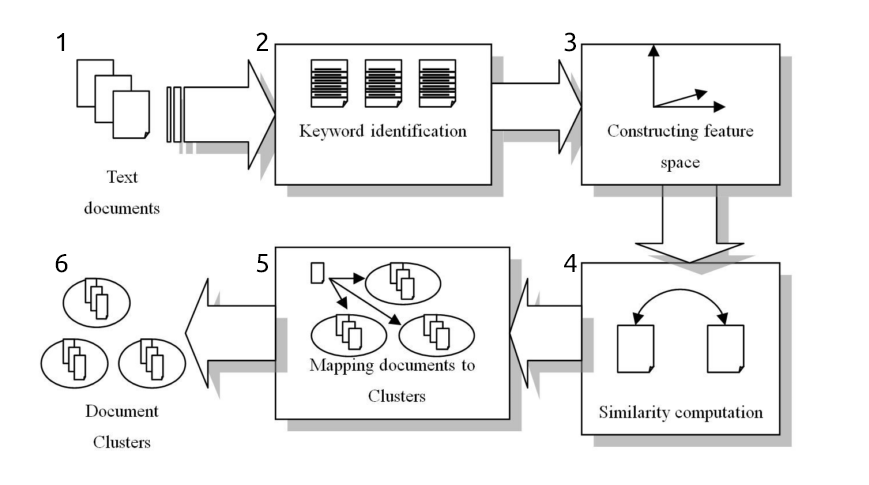
\includegraphics[width=12cm]{images/1_Text_Clustering_Main_Framwork.png}
  \end{center}
  \caption{ Text Clustering Main Framework from \citet{Dozono2012} }
  \label{fig:1_Text_Clustering_Main_Framwork}
\end{figure}
In the first step a data set must be provided in order to cluster the documents. 
The second step "Keyword identification" is where non relevant words are removed from the documents. \citet{Kang2003} proves that keyword removal improves clustering. Another way to extract features is to differentiate text features by analizing the document corpora. For example if the dataset is composed from HTML or XML documents it is possible to identify more relevante features due to the characteristics of the markup. In \ref{sub:topic_detection_on_twitter} it will be described twitts characteristics as a document and in \ref{sec:architecture} how feature extraction will be implemented on this project.
"Constructing the Feature Space" is characterized by converting the keywords of each document into vectors, the most common algorithm used for this task is SVM (Support Vector Machines). In SVM each vector dimension means one detected key word and each document is represented by the vector of keywords in the feature space. This process and keyword removal is described in Figure \ref{fig:2_svm}.
Due to the way documents are represented in SVM it is normal that vectors become very large and full of zeros ( keywords not present) and it is needed to use sparse vectors to represent the documents in a more efficient way.

\begin{figure}
  \begin{center}
    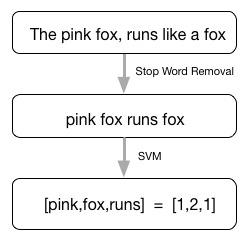
\includegraphics[width=5cm]{images/2_svm.jpg}
  \end{center}
  \caption{ Stop word removal and transformation to Vector Space Model }
  \label{fig:2_svm}
\end{figure}

Dimensional reduction is done after the construction of the vector space model, in order to reduce the size of the vector space. There are two main ways to do this PCA (Principal Component Analysis) and LSI (Latent Semantic Indexing). PCA calculates the k eigenvectors of the co-variance of the document matrix, which reduces the size of the matrix to k. LSI (Latent Semantic Indexing) works just like PCA but the eigenvectors are calculated directly from the document matrix.

There are two main strategies for Document Clustering, Complete strategie where the data set does not change and Incremental where initial number of document can increase by adding new documents. After a new document is added it can be merged into a existing cluster, or can be separated as a new category. While adding new documents it might be needed to re run the clustering algorithm. 

After the algorithm converges, cluster similarity can be calculated in multiple ways:
\begin{itemize}
  \item Shortest Distance Method: Shortest distance between two members of different clusters.
  \item Longest Distance Method: Longest distance between two members of different clusters.
  \item Group Average Method: The average distance between all elements of both clusters.
  \item Centric Method: The distance between the center of two clusters.
\end{itemize}

There many clustering algorithms, here we will focus on the three most popular.K-means works by randomly selecting k documents as the cluster centroids, then assign each document to the nearest centroid, and finally recalculate the the centroid with new added documents. The algorithm should be executed until convergence which reflects in the centroids stop changing. K-means has the advantage that the number of centroids must be selected before starting the algorithm.
AHC or Agglomerative Hierarchical Clustering is hierarquical clustering algorithm where clusters have sub-clusters which have subclusters. Like K-means it is also a simple algorithm that starts by calculating the similarity matrix, then each document is seen as a cluster and finally merge the nearest two clusters into one and update the similarity matrix. The algorithm ends when there is only one cluster or due to clustering entropy.An AHC classic example is species taxonomy where species have subspecies which have subspecies, etc.
Lastly there is Self-organizing Maps introduces by \citep{Kohonen1990} which will be used in the thesis and will be detailedly described in the next subsection \ref{sub:self_organizing_maps}.


% subsection clustering (end)

\subsection{The Self-organizing Map} % (fold)
\label{sub:the_self_organizing_map}

The Self-organinzing map, or for short SOM is a kind of recurrent artificial neural network that as the desired property of topology preservation which mimics the way cortex of high developed animals brains work.

As \citep{Bacao2005} describes the basic idea behind SOM is to map the data patterns into an n-dimensional grid of neurons or units. That grid is also know as the output space, as opposed to the initial space also called input space, where the input patterns are. Both spaces can be seen in picture \ref{fig:5_neighbours_converge}.

SOMs work similar to the way that is thought that the human brain works by having a set of neurons that through learning experience specialize in the identification of certain types of patterns. These so called neurons are responsible for categorizing input patterns for which they are responsible. Nearby neurons will be organized by similarity which will cause that similar patterns will activate in similar areas of the SOM.
With a topology preserving mapping, SOM organizes the information spatially where similar concepts are mapped to adjacent areas. The topology is preserved in a sense that as far as possible neighborhoods are preserved through the mapping process.
Neurons are displayed in an n dimensional grid, generally rectangular, but other dimensions are possible like hexagonal or octagonal.  The grid of neurons, also called output space can be divided in neighborhoods where neurons responsible for the same kind of input reside.
In SOM neurons will have the same amount of coefficients as the input patterns and can be represented as vectors through the SVM model described earlier in section \ref{sub:clustering}.

Before describing the algorithm it is important to define three key aspects of the SOM, the learning rate and quantization error. The learning rate is a function that will be decreased in order to converge to zero, it will be applied to winning neurons and their neighbors in order for them to move toward the corresponding input pattern. Quantization Error is the distance between a given input pattern and the associated winning neuron, it describes how well neurons represent the input pattern. The radius of the neighborhood around the winner neuron is particularly relevant to the totpology of the SOM, deeply afecting the unfolding of the output space as stated by \citep{Bacao2005} 
The learning phase is characterized by the training algorithm, which works the following way:
\begin{itemize}
  \item Neurons can be initialized randomly or it is possible to select initialization neurons.
  \item Given an input pattern, calculate the distance between the input pattern and every neuron on the network.
  \item The winning neuron will be the closest neuron to the input pattern.
  \item The neuron will move towards the data pattern at a given learning rate, in order to improve his representation as can be seen in figure \ref{fig:4_wining_neuron_converge}.
  \item Neighbor neurons will also improve their representation in order to keep the network progressively organized as can be seen in figure \ref{fig:5_neighbours_converge}.
\end{itemize}

\begin{figure}
  \begin{center}
    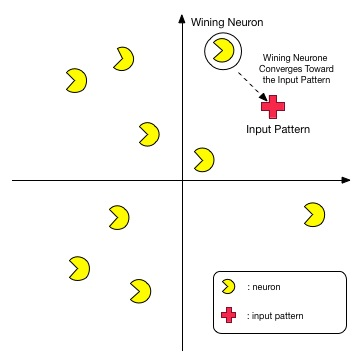
\includegraphics[width=5cm]{images/4_wining_neuron_converge.jpg}
  \end{center}
  \caption{ Winning neuron converging at learning rate }
  \label{fig:4_wining_neuron_converge}
\end{figure}

\begin{figure}
  \begin{center}
    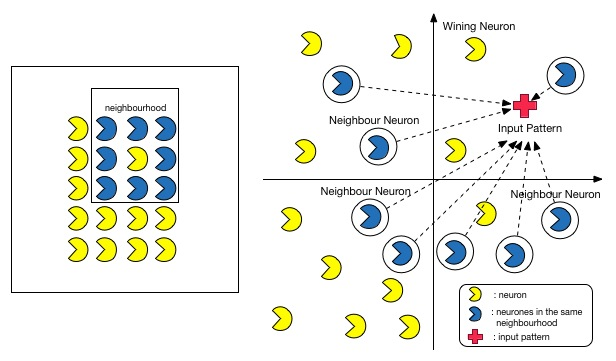
\includegraphics[width=12cm]{images/5_neighbours_converge.jpg}
  \end{center}
  \caption{ On the left the output space neighbor, on the right the neighbors of the winning neuron converging }
  \label{fig:5_neighbours_converge}
\end{figure}

After the algorithm converges, the prediction phase starts. On the prediction phase new input patterns can be quickly assigned to the SOM, without need to apply the learning rate to the winning neuron and his neighbors (the learning rate converged to zero), it very easy and fast to classify new data now. It is possible that during training the SOM gets stuck while unfolding, this kind of behavior might happen if the input patterns are very complex.

In order to visually interpretate the result of the SOM U-matrices may be used as stated by \citep{Bacao2005}. The U-matrix is a representation of the SOM in which distances, in the input space between neurons is represented using a gray scale.

The advantages of using SOM is data noisy immunity, easy to visualize the data and parallel processing.

% subsection the_self_organizing_map (end)


%!TEX root = ../projecto.tex
\section{Related Work} % (fold)
\label{sec:related_work}

\subsection{Self-Organizing Maps} % (fold)
\label{sub:self_organizing_maps}
% subsection self_organizing_maps (end)


\subsection{Topic Detection on Twitter} % (fold)
\label{sub:topic_detection_on_twitter}
% subsection topic_detection_on_twitter (end)
% section related_work (end)


\begin{itemize}
  \item What did we know about the problem before I did this study? 
  \item What did we do different from previous works? 
  \item Discuss the relevant primary research literature 
  \item Works should be organized by their relevant characteristics 
  \item Comment on why it is relevant for your work 
  \item Comment on what your work does differentely 
\end{itemize}
%!TEX root = ../projecto.tex

\section{Architecture} % (fold)
\label{sec:architecture}
This Section is comprised of the multiple layers needed in order to successfully be able to implement the proposed project objectives described in subsection \ref{sub:objectives}. In subsection \ref{sub:data_gathering} will be discussed the data gathering process, the at subsection \ref{sub:implementing_the_som} will be detailed the SOM algorithms that will be tried in order to achieve the best results in Topic Detection on Twitter. The description of results evaluation will be described in subsection \ref{sub:testing_results} and finally the Web Site architecture will be described in subsection \ref{sub:web_site_creation}.

\subsection{Building a Dataset} % (fold)
\label{sub:data_gathering}
In order to apply any kind of Clustering or Learn to Rank algorithm, a Data Set is needed. The two most common approaches to Dataset building are finding some Dataset that was used beforehand by someone, use the Twitter API to build your own or any combination of the two. For this project we will focus on building our own dataset for SOM training, but existing datasets might be used in order to rate results. The description of existing datasets will be presented in Subsection~\ref{sub:testing_for_precision_and_recall}. 

\subsubsection{Twitter API} % (fold)
 \label{ssub:building_a_data_set}
 Building your own Data Set through the Twitter API has become harder with passing years with the introduction of API limits and mandatory authentication. With these new limitations, companies like gnip \footnote{http://gnip.com/topsy/} or \footnote{http://www.tweetarchivist.com/about/subscriptions} with licenses from Twitter are selling access to their archives of tweets.

 In order to retrieve data from Twitter is crucial to understand how their API functions. The Twitter API right now is divided into two, the REST API and the Streaming API. Both of the API's can be used at the same time, and have different types of limits. In a general way, the streaming API is used for subscriptions, where a an application can subscribe a given hashtag or User activity on the social network, and they are automatically pulled to the subscriber app. The Streaming API has no specific limit being described in the docs as "The public streaming APIs cap the number of messages sent to your client to a small fraction of the total volume of Tweets at any given moment" \footnote{https://dev.twitter.com/docs/faq\#6861}.

 The REST API works by requesting resources and getting the results in a restful way. Here the limits are strict, an application cat only get a maximum number of 3200 Tweets per user and 180 calls to the API per 15 minutes, more API limits can be found on the Twitter API Documentation \footnote{https://dev.twitter.com/docs/rate-limiting/1.1/limits}.
 % subsubsection building_a_data_set (end) 

\subsubsection{Crawling Twitter} % (fold)
\label{sub:crawling_twitter}
In order to get tweets from the Twitter API, the data will be crawled in a breath-first fashion where the first user can be selected randomly:

\begin{itemize}
  \item Get all Tweets from the user.
  \item Get user profile info.
  \item Get list of followers/followees.
  \item Select a follower/followee and repeat step one.
\end{itemize}

The algorithm will stop at a given depth level, also if API limits are exceeded the algorithm will have to stop for 15 minutes and afterwards resumed. Given the API access limits, there will be no need to run the crawler asynchronously since achieving a greater level of performance will only make the algorithm achieve API limits sooner.
% subsubsection crawling_twitter (end)

\subsubsection{Storing Crawled Data} % (fold)
\label{sub:storing_crawled_data}
While the crawler is getting data from Twitter, it will be storing it in a Redis database \footnote{http://redis.io/}. Given the amount of databases available in last few years, Redis was chosen for this project because it met the following criteria:
\begin{itemize}
  \item Free.
  \item Simple to install and run. 
  \item Can persist data to disk.
  \item Its really fast to write, by not granting data integrity (which is not a problem since this project is not dealing with sensitive information)
  \item Good documentation.
  \item Non relational, Key/Value store.
  \item Stores json.
  \item Client libraries for almost every programing language.
  \item Integrated publish/subscriber.
\end{itemize}

Given the characteristics of the Redis database, there will be no need to write a schema beforehand. With this in mind, user information and Tweets will be stored directly in json into the Database.
% subsubsection storing_crawled_data (end)
% subsubsection data_gathering (end)

\subsection{The SOM Algorithm} % (fold)
\label{sub:implementing_the_som}
The SOM algorithm in this report will have a twofold approach. Primarily it will be tried to transform the tweet social characteristics and words into a vector using the vector space model, this approach will use the default SOM implementation and will be described in detail in Subsection~\ref{ssub:default_som_approach_}. The second approach will be inspired by \citet{Bacao2005} where the SOM algorithm will be altered in order to take in consideration the social network during the its training, this implementation will be described in Subsection~\ref{ssub:social_som}.
% subsection implementing_the_som (end)

\subsubsection{Default SOM Approach } % (fold)
\label{ssub:default_som_approach_} In order to train the SOM first it will be needed to convert the tweets into the vector space model. There will be two binary vectors, the first one will represent the presence of all the words gathered in all tweets where each value 1 will  represent the presence of a word. The second vector will represent the social connections between the user. On a first approach in order to  give more relevance to social connections only followers that are followed back will be represented with ones, this approach will give a higher representation to the social interaction between the two users since on the Twitter social network it possible to follow someone without the followed person accept the request. In the end both vectors, the word representation vector and the social connections representation vector will be concatenated. Figure~\ref{fig:vsm} shows the transformation from the tweet into the vector space model. 

\begin{figure}[tb]
  \begin{center}
    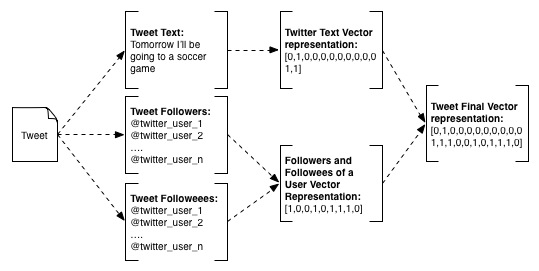
\includegraphics[width=9cm]{images/10_tweet_svm_transform.jpg}
  \end{center}
  \caption{Vector Space Transformation of a Tweet}
  \label{fig:vsm}
\end{figure}

The SOM initialization will be tried in different ways and measured to see which gives the best results. The initialization characteristics will be the following:
\begin{itemize}
  \item Random initial number of neurons with random content.
  \item Random initial number of neurons with random content evenly distributed.
  \item Each neuron will be the representation of each user that was crawled.
  \item Each neuron will be comprised of words relevant to a determined topic, and will be responsible to categorize that topic.
  \item Each neuron will be the representation of a user that is relevant to determined topic, for example the user \emph{Optimus Alive} would be responsible for categorizing the topic \textit{"Music Festivals"}  while \emph{Cristiano Ronaldo} neuron representation would be responsible for detecting the topic \emph{Soccer}.
\end{itemize}

In the initialization ways described above, only the last two will give a SOM ready to classify. The first three options would build uncategorized clusters that would have to be classified \emph{a posteriori}, nevertheless it would be important to look at the results given by them because they could be more interesting then the results from the last two items.
% subsubsection default_som_approach_ (end)

\subsubsection{Social SOM} % (fold)
\label{ssub:social_som}
In this approach, the use of the vector that described the followers/followees of the user that created the tweet, which is described  in Subsection~\ref{ssub:default_som_approach_} will be discarded. Instead there will be a new vector that describes the number of hops between twitter users, a visual representation of this vector can be seen in Figure~\ref{fig:hops}.
By modifying the SOM training algorithm, input patterns will only be measured against neurons that have a determined level of social affinity. This social affinity will be defined as \(x\) which will define the number of followers/followees relations will be applied. For example if \(x = 1\) only neurons that belong to a follower/followee will be selected for comparison to find which is the winning neuron. If \(x = 2\) not only the followers/followees of a user will be selected for comparison, but also the followers/followees of the followers/followees. Finally if \(x\) would be equal to the number of users used in the dataset, then all neurons would be used for comparison, making this solution equal to a normal SOM.

\begin{figure}[tb]
  \begin{center}
    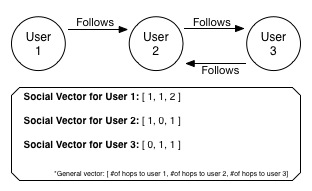
\includegraphics[width=8cm]{images/11_hops_svm.jpg}
  \end{center}
  \caption{Vector describing the number of hops between followers}
  \label{fig:hops}
\end{figure}
% subsubsection social_som (end)
\subsubsection{SOMS Development} % (fold)
\label{ssub:soms_development}
The development and testing of the SOM described in Sub-subsection~\ref{ssub:social_som} and Sub-subsection~\ref{ssub:default_som_approach_} will be completely independent of the Web Site described in Subsection~\ref{sub:web_site_creation}. The SOM training will be made using the datasets described in Subsection~\ref{sub:crawling_twitter} and connection with components from the Web Site will be made through the Publish/Subscriber Redis interface. This approach will create an highly modular solution where it will be possible to interact with the trained SOM through terminal where it will be possible to visualize and test results.

% subsubsection soms_development (end)
\subsection{Web Site} % (fold)
\label{sub:web_site_creation}
As described in the report objectives a web site will created to demonstrate the project categorizing tweets per topics. In order to achieve this a Web Application will be implemented that works in the following way:
\begin{itemize}
  \item A user will be able to login with his twitter id.
  \item The browser will start displaying the user tweets, with the associated topic.
  \item After all the user tweets are displayed, some statistics about the user tweeting topics will be displayed.
\end{itemize}
The wire-frames for the application are provided as attachment, the architecture of the solution can be seen in Figure~\ref{fig:solution} and will be described in the following sub-subsections.
\begin{figure}[tb]
  \begin{center}
    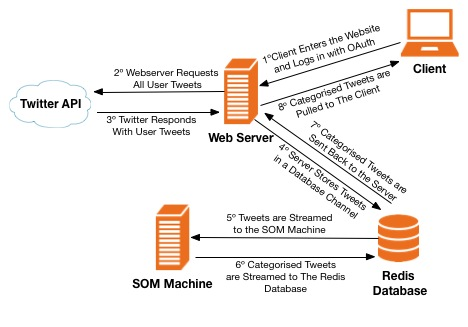
\includegraphics[width=9cm]{images/12_network.jpg}
  \end{center}
  \caption{Topology of the Solution}
  \label{fig:solution}
\end{figure}

\subsubsection{Client Side Application} % (fold)
\label{ssub:client_side_application}
The client side application will be running on the browser of whomever connects to the website, on the client browser. This application is responsible to authenticate itself against the Twitter API through OAuth and after that will be establishing a web-socket channel that will be receiving the categorized tweets has soon as the server dispatches them. The client application will also have to display an interface to the user so he can interact with the application.
% subsubsection client_side_application (end)

\subsubsection{Web Server} % (fold)
\label{ssub:web_server}
The web server will be very simple, it will only have to get the tweets from the Twitter API and publish them in a channel through the Redis Publish/Subscriber interface, on the other side the SOM machine will be receiving the Tweets and categorizing them. Also the web server will have to subscribe to the channel where the SOM Machine is publishing the categorized tweets in order to be able to push them to the client through web-sockets.
% subsubsection web_server (end)

\subsubsection{Redis Database} % (fold)
\label{ssub:redis_database}
The Redis database will be used as a middle man between the Web Server and the SOM Machine as publish/subscriber system. This is extremely useful because it will separate the login of the web server and web application from the rest of this project. In this way the SOM machine can be running the topic categorization in any programing language while the server can also be working in another language and still be able to contact each other in a simple and efficient way.
% subsubsection redis_database (end)

\subsubsection{SOM Machine} % (fold)
\label{ssub:som_machine}
The SOM Machine is where the Self-organizing Map trained with the crawled data described in Subsection~\ref{sub:crawling_twitter} will be functioning. It will be subscribing to new tweets sent from the Web Server and will categorize them using the previously trained SOM. After the tweets are categorized they will be published back so the Web Server can deliver them to the client.
% subsubsection som_machine (end)

\subsubsection{Solution Overview} % (fold)
\label{ssub:solution_overview}
In this Sub-subsection will reside the description of how everything in this solution fits together, based on the diagram in Figure~\ref{fig:solution} and the steps described will be the same, but they will have more detail. For simplicity sake the OAuth authentication from the client to the twitter API will be omitted since its only objective is to get access to the user tweets.

\begin{itemize}
  \item \textbf{First Step} The client connects to the website through the browser and will login with his twitter account in order for the server be able to download all of his Tweets. When the login process is over it keep an open web-socket with the server in order to receive the categorized tweets.
  \item \textbf{Second and Third Step} The web-server will request all the user tweets through the Twitter API. Twitter will respond with all \footnote{The number of tweets per user are limited to the 3200 most recent through the twitter API} the tweets from the user that logged in.
  \item \textbf{Forth and Fifth Step} The web server will publish the tweets in the Redis database, while is subscribing to the channel where the categorized tweets will come out. On the other side the SOM Machine is subscribing to the uncategorized tweets in order to categorize them.
  \item \textbf{Sixth and Seventh Step} After the SOM machine categorizes the tweets it will publish them to the Redis database, which is being subscribed by the web server.
  \item \textbf{Eight Step} As soon as categorized tweets start hitting the server they will be immediately sent to the client through web sockets. On the client as soon as the categorized tweets hit the browser, they will be injected into the DOM and the user will start to see the tweets that he has made categorized in topics. Lastly after all the tweets have been sent to the browser, some statistics will appear with the amount of tweets per topic throughout the time.
\end{itemize}
% subsubsection solution_overview (end)

% section architecture (end)
 
%!TEX root = ../projecto.tex

\section{Evaluation Metrics} % (fold)
\label{sec:evaluation_metrics}

% section evaluation_metrics (end)

\begin{itemize}
  \item How am I gonna evaluate my work?
\end{itemize}

\subsection{Evaluation Criteria by Teachers} % (fold)
\label{sub:evaluation_criteria}
\begin{itemize}
  \item Ability to understand the research problem
  \item Clear and well defined goals
  \item Description of the different approaches explored
  \item Ability to relate the state-of-the-art with the research theme Work methodology and adequate planning for the next stage Organization and quality of the written document
  \item Inclusion and completeness of updated and appropriate references Oral presentation and discussion
\end{itemize}
% subsection evaluation_criteria (end)
%!TEX root = ../projecto.tex

\section{Conclusions and Future Work} % (fold)
\label{sec:coclusions_future_work}

% section coclusions_future_work (end)

%!TEX root = ../projecto.tex

\section{Attachments} % (fold)
\label{sec:attachments}

\subsection{Web Site Wire-frames} % (fold)
\label{sec:web_site_wire_frames}
\begin{figure}[tb]
  \begin{center}
    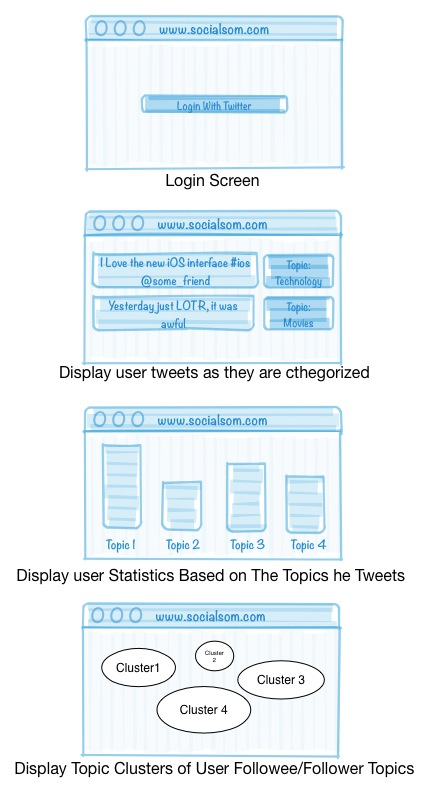
\includegraphics[width=10cm]{images/9_wireframes}
  \end{center}
  \caption{Website to display user Twitter content}
  \label{fig:wireframes}
\end{figure}

% section web_site_wire_frames (end)

% section attachments (end)

\bibliographystyle{plain}
\bibliography{/Users/bersimoes/Documents/Tese/PaperProjecto/Bibtex/library,/Users/bersimoes/Documents/Tese/PaperProjecto/Bibtex/Sites}

\end{document}
